\chapter{PSO on benchmark functions}
\section{Introduction}
In this section we will give the formulation of all the benchmark functions we have implemented for the developed PSO to optimize. The functions vary from being relatively easy to optimize, to functions that contain lots of local minima and a slightly concealed global minmima. In total we will formulate 14 benchmark functions.

The reason why these functions have variate amount of local and global minima, it to test various factors on how good the algorithm is that is being applied on the function. The factors that are tested are:
\begin{itemize}
\item Rate of convergeance
\item Exploration
\item Exploitation
\item Diversity
\item Breaking out of local minima
\item Information sharing
\end{itemize}

The benchmark functions were chosen because of their extensive use in the literature. For each new optimization algorithm these functions are used to showcase how good the algorithm is with regard to optimisation.

The functions have known global optima and local optima, which means researchers are able to produce statistical information on how the algorithm performs. For instance, researchers will not be able to measure accurately the performance of the algorithm on a NP-Complete problem. Yes, they can compare results with what other algorithms have produce, but cannot with absolute certain say or measure the algorithm convergence,diversity etc. 

With these benchmark functions, their optima are mathematically determined. Thus, researchers can now with sureity measure the convergence rate, diversity and compare it with other algorithms, since the domain the algorithms operate it is not as specific as a NP-Complete problem. Rather, the domain is mathematical and deterministic and therefore allows easy comparison.

To measure the performance of the PSO algorithm, two variants have been developed. One normal PSO that uses the original PSO algorithm and then a second PSO which utilizes the notion of inertia to move particles. These two algorithms will be applied to all the benchmarks presented in the next section.

In the next section, all the benchmarks that will be used for testing the PSO algorithms will be formulated. Followng the test function section, a section will be presented that shows that 3D graphs of these functions. This chapter will concluded with the results sections where the results of the PSO algorithms that were developed are presented as well as compared with other results that have been presented in the literature
\subsection{Test Functions}
\textbf{Development of a parallel optimization method based on genetic simulated annealing algorithm}\\
\textbf{Adaptive Diversity in PSO}\\
\textbf{A hybrid intelligent genetic algorithm}\\
\textbf{A Diversity-Guided Particle Swarm Optimizer – the ARPSO}\\
\textbf{A distributed hierarchical genetic algorithm for efficient optimization and pattern matching}\\
\textbf{Tabu search for global optimization of continuous functions with application to phase equilibrium calculations}\\
\textbf{Tabu Search applied to global optimization}\\
\textbf{On the performance of artificial bee colony (ABC) algorithm}\\
\textbf{Improving solution characteristics of particle swarm optimization using digital pheromones}\\
\textbf{Continuous ant colony system and tabu search algorithms hybridized for global minimization of continuous multi-minima functions}\\
\textbf{Chaotic bee colony algorithms for global numerical optimization}\\
\textbf{A powerful and efficient algorithm for numerical function optimization: artificial bee colony (ABC) algorithm}\\
\textbf{A New Quantum Behaved Particle Swarm Optimization}\\
\textbf{A comparative study of Artificial Bee Colony algorithm}\\
\subsubsection{DeJong F1 Function}
\begin{equation}
\label{eq:DeJongF1}
	f(x) = \sum_{i=1}^n x^2_i, -5.12 \leq x_i \geq 5.12, i \in \mathbb{N}
\end{equation}
The DeJong F1 Function has the following global minium when $f(x) = 0, x(i) = 0, i:n$ where $n$ is the amount of dimensions. 
\subsubsection{Shekel's Foxhole}
\begin{align}
	f(x_1,x_2) &= \{0.002 + \sum^{25}_{j=1} [j + (x_1 - a_{1j})^6 + (x_2 - a_{2j})^6]^{-1}\}^{-1}\\
\intertext{where}
	a &= \begin{pmatrix} \nonumber
			-32 & -16 & 0 & 16 & 32 & -32 & ... & 0 & 16 & 32 \\
			-32 & -32 & -32 & -32 & -32 & -16 & ... & 32 & 32 & 32 \\
		 \end{pmatrix}
\end{align}
the variables $x_1$ and $x_2$ are usually restricted to the square represented by $-65.356 \leq x_1 \leq 65.357, -65.357 \leq x_2 \leq 65.356$. The global optimum is when $f(x_1,x_2) = 0, \{x_1,x_2\} = \{-32,-32\}$
\subsubsection{Rastrigin}
\begin{equation}
	f(x) = 10n + \sum_{i=1}^n [x_i^2 - 10\cos(2 \pi x_i)],\, i \in \mathbb{N}
\end{equation}
The values of the variable $x_i$ is bounded by the hypercube $-5.12 \leq x_i \leq 5.12$. The global optimum for the function is when $f(x_i) = 0,\, x_i = 0, \, i = 1,\dots,n$
\subsubsection{Schwefel}
\begin{equation}
	f(x) = 418.9829n - \sum^n_{i=1} [x_i\sin{\sqrt{|x_i|}}], \qquad i \in \mathbb{N}
\end{equation}
The variable $x_i$ is restricted to be in the hybercube $-500 \leq x_i \leq 500, i = 1,\ldots,n$. The global optimum for the function is $f(x) = 0$ when $x_i = 420.9687$.
\subsubsection{Griewank}
\begin{equation}
	f(x) = \sum^n_{i=1} \frac{x^2_i}{4000} - \prod^n_{i=1}\cos{(\frac{x_i}{\sqrt{i}})} + 1, \qquad i \in \mathbb{N}
\end{equation}
The variable $x_i$ is bounded to within the hypercube $ -600 \leq x_i \leq 600 $. The global optimum of the function is when $f(x) =0$ which occurs when $ x_i = 0, i = 1, \dots, n $
\subsubsection{Salomon}
\begin{equation}
	f(x) = -\cos{(2\pi\sum_{i=1}^n\sqrt{x_i^2})} + 0.1 \sqrt{\sum_{i=1}^n x_i^2} + 1, \quad i \in \mathbb{N}
\end{equation}
Unlike the previous functions discussed in this section, the Salomon function imposes no constraint on the $x_i$ variable. The global optimum is when $f(x) = 0$ and $x_i = 0$ where $i = 1,\ldots,n$
\subsubsection{Ackley}
\begin{equation}
	f(x) = -20e^{-0.2\sqrt{\frac{1}{2}\sum_{i=1}^n x_i^2}} - e^{\frac{1}{2}\sum_{i=1}^n\cos{2\pi x_i}} + 20 + e^1, \qquad i \in \mathbb{N}
\end{equation}
The variable $x_i$ is restricted to the hypercybe represented by $-32.768 \leq x_i \leq 32.768$. The global minimum is when $f(x) = 0$ and is obtainable for $x_i = 0, i = 1,\ldots,n$.
\subsubsection{Six-Hump Camel Back}
\begin{equation}
	f(x_1,x_2) = (4 - 2.1x_1^2 + x_1^{\frac{4}{3}})x_1^2 + (x_1x_2) + (-4 + 4x_2^2)x_2^2
\end{equation}
The variables $x_1$ and $x_2$ are subject to the following boundary constraints $-3 \leq x_1 \leq 3$ and $-2 \leq x_2 \leq 2$. The global minimum is when $f(x_1,x_2) = -1.0316$ and is obtained when $x_1 = -0.0898$ and $x_2 = 0.7126$
\subsubsection{Shubert}
\begin{equation}
	f(x_1,x_2) = -\sum_{i = 1}^5 (i\cos{(i +1)x_1 + 1})\sum_{i=1}^5 (i\cos{(i+1)x_2 + 1})
\end{equation}
The search domain constrained to $-10 \leq x_i \leq 10, i = 1,2, \ldots, n$. The global optimum which is when $f(x_i) = -186.7309$.
\subsubsection{Himmelblau}
\begin{equation}
	f(x_1,x_2) = (x_1^2 + x_2 - 11)^2 + (x_1 + x_2^2 - 7)^2
\end{equation}
The variables $x_1,x_2$ are constraint to be within the hypercube represented by $-6 \leq x_1 \leq 6, -6 \leq x_2 \leq 6$. The Himmelblau function contains no local optima, but on the contrary, it has 4 global optima when $f(x_i) = 0$ which can be obtained at the following points $(x_1,x_2) \in \{(-3.779310,-3.283185),(-2.805118,3.131312),(3,2),(3.584428,-1.848126)\}$
\subsubsection{Rosenbrock Valley}
\begin{equation}
	f(x) = \sum_{i=1}^{n-1}[100(x_{i+1} - x_i^2)^2 + (1-x_i)^2
\end{equation}
The variable $x_i$ is bounded to with the following constraint $ -2.048 \leq x_i \leq 2.048 $. The global optimum is when $f(x) = 0$ and is obtained when $x_i = 1, i = 1,\ldots,n$.
\subsubsection{Dropwave}
\begin{equation}
	f(x) = -\frac{1 + \cos{(12\sqrt{x_1^2 + x_2^2})}}{\frac{1}{2}(x_1^2 + x_2^2) + 2}
\end{equation}
The variables $x_1$ and $x_2$ are restricted to be within the following bounds $-5.12 \leq x_i \leq 5.12$
The variables $x_1$ and $x_2$ are restricted to be within the following bounds $-5.12 \leq x_i \leq 5.12$
\subsubsection{Easom}
\begin{equation}
	f(x_1,x_2) = -\cos(x_1)\cos(x_2)e^{(-(x_1 - \pi)^2 - (x_2 - \pi)^2)}
\end{equation}
The variables $x_1$ and $x_2$ are restricted to be within the hypercube represented by $-100 \leq x_1 \leq 100, -100 \leq x_2 \leq 100$. The global minimum is when $f(x_1,x_2) = -1$ and is obtainable if $(x_1,x_2) = (\pi,\pi)$
\subsubsection{Branins}
\begin{align}
	f(x_1,x_2) &= a(x_2 - bx_1^2 + cx_1 - d)^2 + e(1-f)\cos{x_1} + e \\
\intertext{where}
	a &= 1\nonumber\\
	b &= \frac{5.1}{4\pi^2}\nonumber\\
	c &= \frac{5}{\pi}\nonumber\\
	d &= 6\nonumber\\
	e &= 10\nonumber\\
	f &= \frac{1}{8\pi}\nonumber
\end{align}
The variables $x_1$ and $x_2$ are subject to the following boundary constraints $-5\leq x_1 \leq 10, 0 \leq x_2 \leq 10$. The global optimum is when $f(x_1,x_2) = 0.397887$ and is obtainable when $x_1$ and $x_2$ have the following values:
\begin{enumerate}
\item $x_1 = -\pi,\:x_2=12.275$
\item $x_1 = \pi,\:x_2=2.275$
\item $x_1 = 9.42478,\:x_2=2.475$
\end{enumerate}
\subsubsection{Michalewicz}
\begin{equation}
	f(x) = -\sum_{i=1}^n\sin{(x_i)}[\sin{(\frac{(1 - x_i^2)}{\pi})}]^{2m}, \qquad i,m \in \mathbb{N}
\end{equation}
The variable $x_i$ is usually constricted to the following defined boundary $0 \leq x_i \leq \pi, i = 1,\ldots,n$. The parameter $m$ defines the steepness of the valleys in the function. The function has two approximated global minima's
%http://www.geatbx.com/docu/fcnindex-01.html#P216_11735
\begin{enumerate}
\item $f(x) = -4.687,\: n = 5$
\item $f(x) = -9.66,\: n = 10$
\end{enumerate}
\subsubsection{Goldstein}
\begin{align}
	f(x_1,x_2) &= (1 + (x_1 + x_2 + 1)^2)\nonumber\\
			   &=*(19-14x_1+3x_1^2 -14x_2 + 6x_1x_2 + 3x_2^2)\nonumber\\
			   &=*(30 + (2x_1 -3x_2)^2\nonumber\\
			   &=*(18 - 32x_1 + 12x_1^2 +48x_2 -36x_1x_2 + 27x_2)\nonumber
\end{align}
The variables $x_1$ and $x_2$ are subject to the following boundary constraints $-2 \leq x_1 \leq 2, -2 \leq x_2 \leq 2$. The function has only global minimum when $f(x_1,x_2) = 3$ and is obtainable when $x_1 = 0$ and $x_2 = -1$
\section{Graphs of Benchmark Functions}
In this section we will present 3D surface and contour graphs for all the mathematical functions discussed in the previous section. These graphs allows one to see the search landscape more visually as well as to comprehend how difficult it is to find the global minima for a particular function.

\subsection{Graphs}
\subsubsection{DeJong's First Function}
~
\begin{figure}[ht]
	\centering
	\setlength \fboxsep{0pt}
	\setlength \fboxrule{0.5pt}
	\fbox{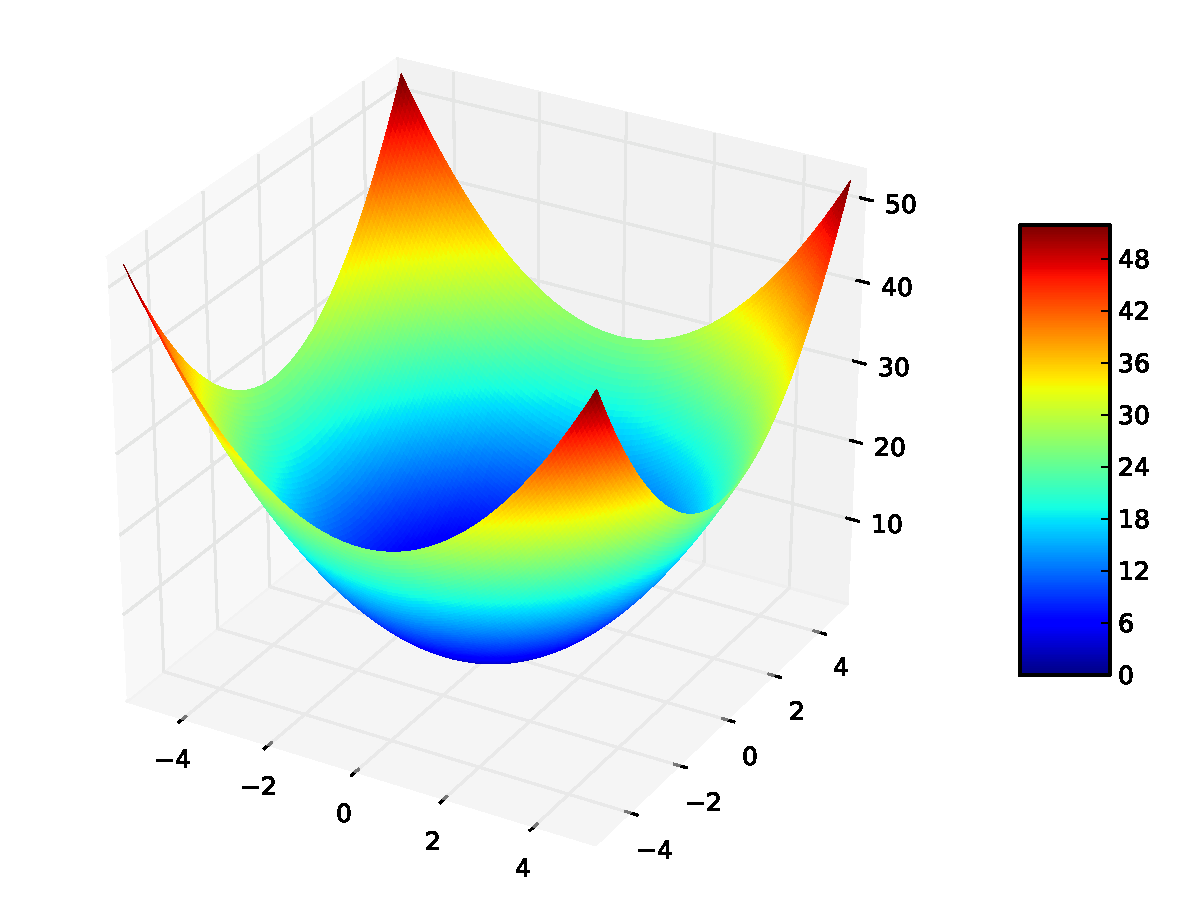
\includegraphics[width=3.0in,height=2.5in]{./Graphs/DeJongF1.pdf}}
	\caption{DeJong's First Function}
	\label{fig:DeJongF1Graph}
\end{figure}
~
\subsubsection{Shekel's Foxhole Function}
~
\begin{figure}[ht]
	\centering
	\setlength \fboxsep{0pt}
	\setlength \fboxrule{0.5pt}
	\fbox{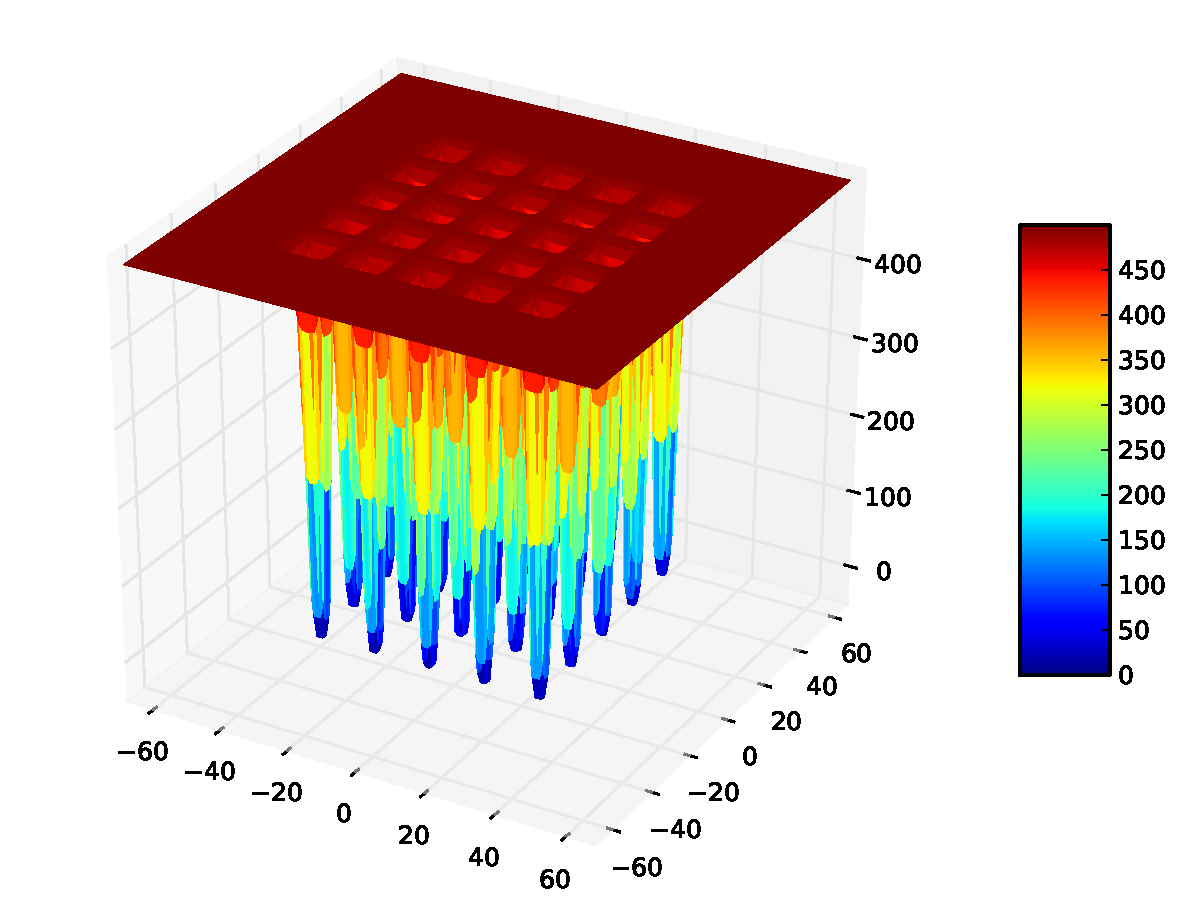
\includegraphics[width=3.0in,height=2.5in]{./Graphs/Shekel.pdf}}
	\caption{Shekel's Foxhole Function}
	\label{fig:ShekelGraph}
\end{figure}
~
\subsubsection{Rastrigin Function}
~
\begin{figure}[ht]
	\centering
	\setlength \fboxsep{0pt}
	\setlength \fboxrule{0.5pt}
	\fbox{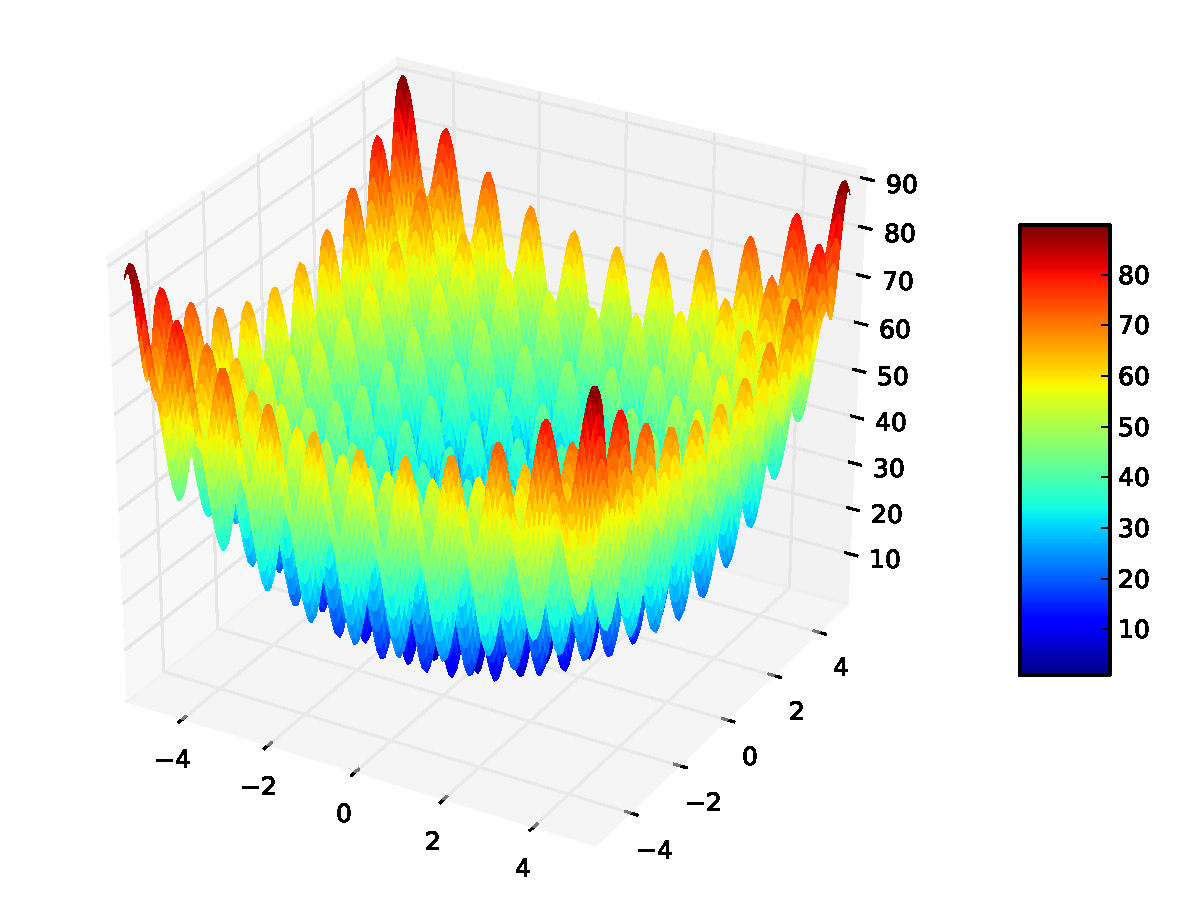
\includegraphics[width=3.0in,height=2.5in]{./Graphs/Rastrigin.pdf}}
	\caption{The Function}
	\label{fig:RastriginGraph}
\end{figure}
~
\subsubsection{Schwefel Function}
~
\begin{figure}[ht]
	\centering
	\setlength \fboxsep{0pt}
	\setlength \fboxrule{0.5pt}
	\fbox{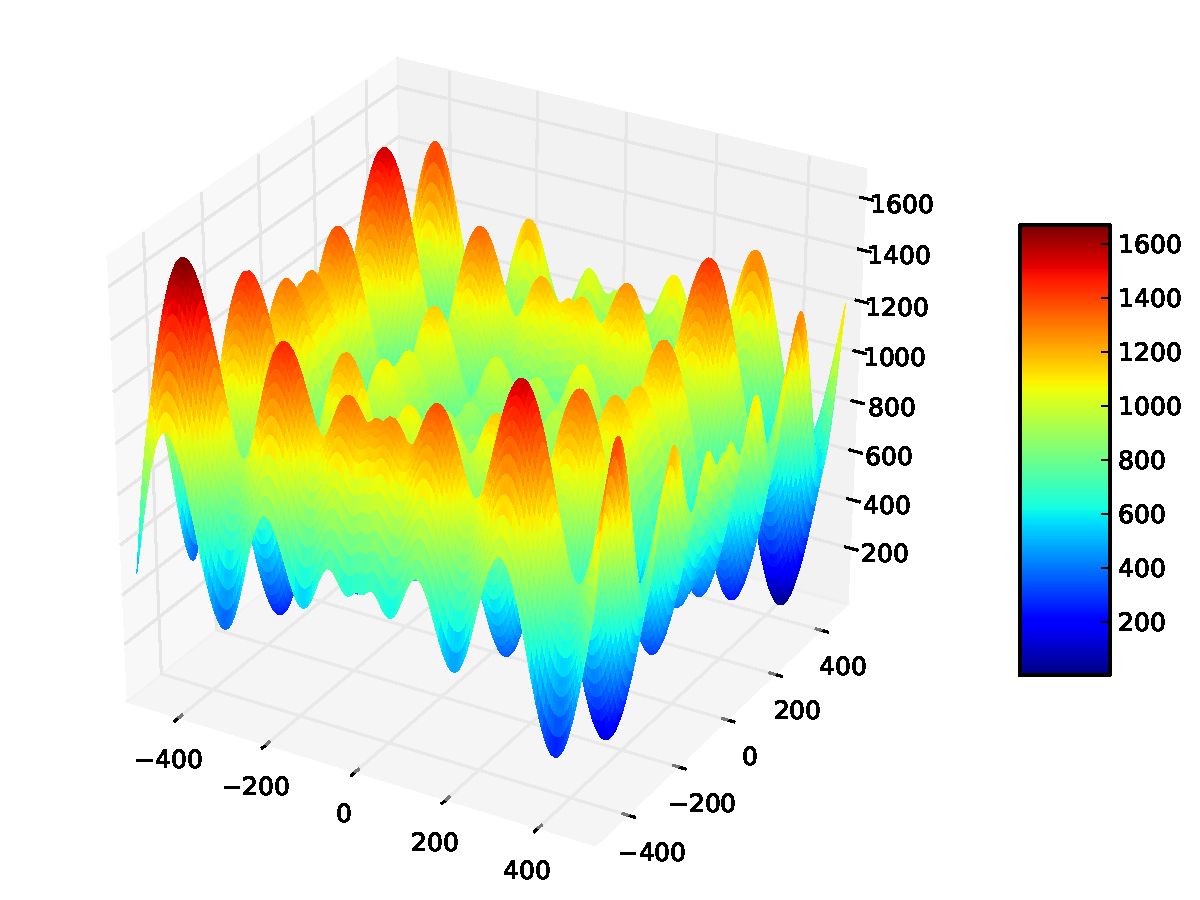
\includegraphics[width=3.0in,height=2.5in]{./Graphs/Schwefel.pdf}}
	\caption{Schwefel Function}
	\label{fig:SchwefelGraph}
\end{figure}
~
\subsubsection{Griewank Function}
~
\begin{figure}[ht]
	\centering
	\setlength \fboxsep{0pt}
	\setlength \fboxrule{0.5pt}
	\fbox{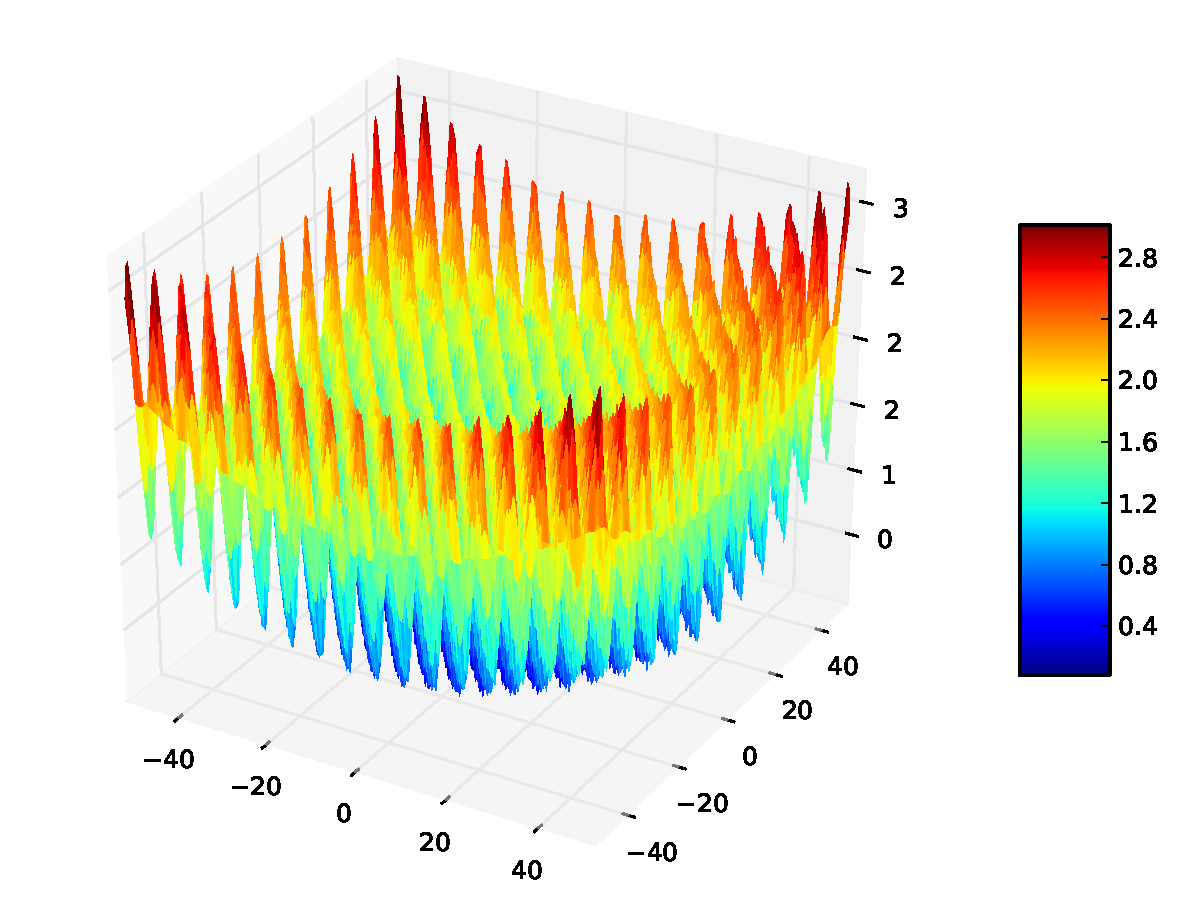
\includegraphics[width=3.0in,height=2.5in]{./Graphs/Griewank_-50_+50.pdf}}
	\caption{Griewank Function}
	\label{fig:GriewankGraph}
\end{figure}
~
\subsubsection{Salomon Function}
~
\begin{figure}[ht]
	\centering
	\setlength \fboxsep{0pt}
	\setlength \fboxrule{0.5pt}
	\fbox{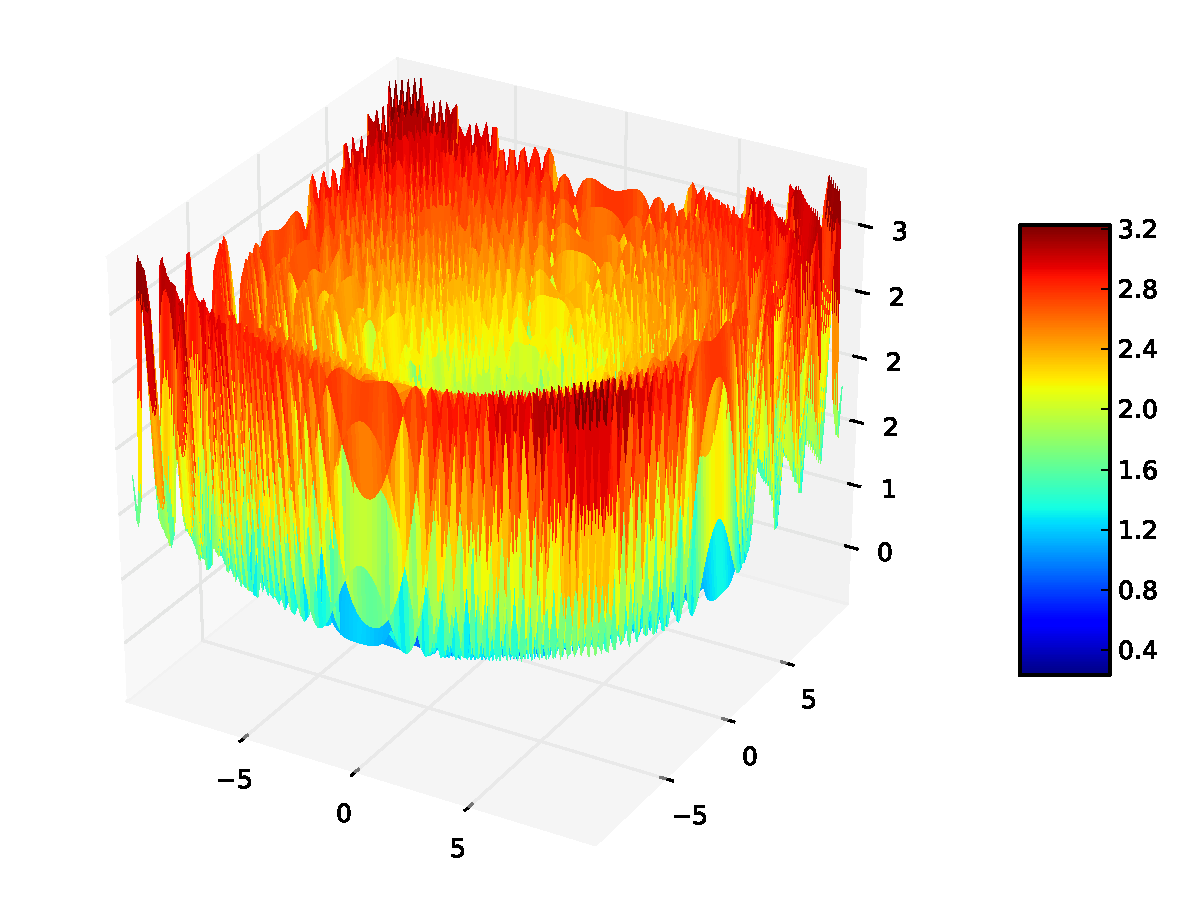
\includegraphics[width=3.0in,height=2.5in]{./Graphs/Salomon_-10_+10.pdf}}
	\caption{Salomon Function}
	\label{fig:SalomonGraph}
\end{figure}
~
\subsubsection{Ackley}
~
\begin{figure}[ht]
	\centering
	\setlength \fboxsep{0pt}
	\setlength \fboxrule{0.5pt}
	\fbox{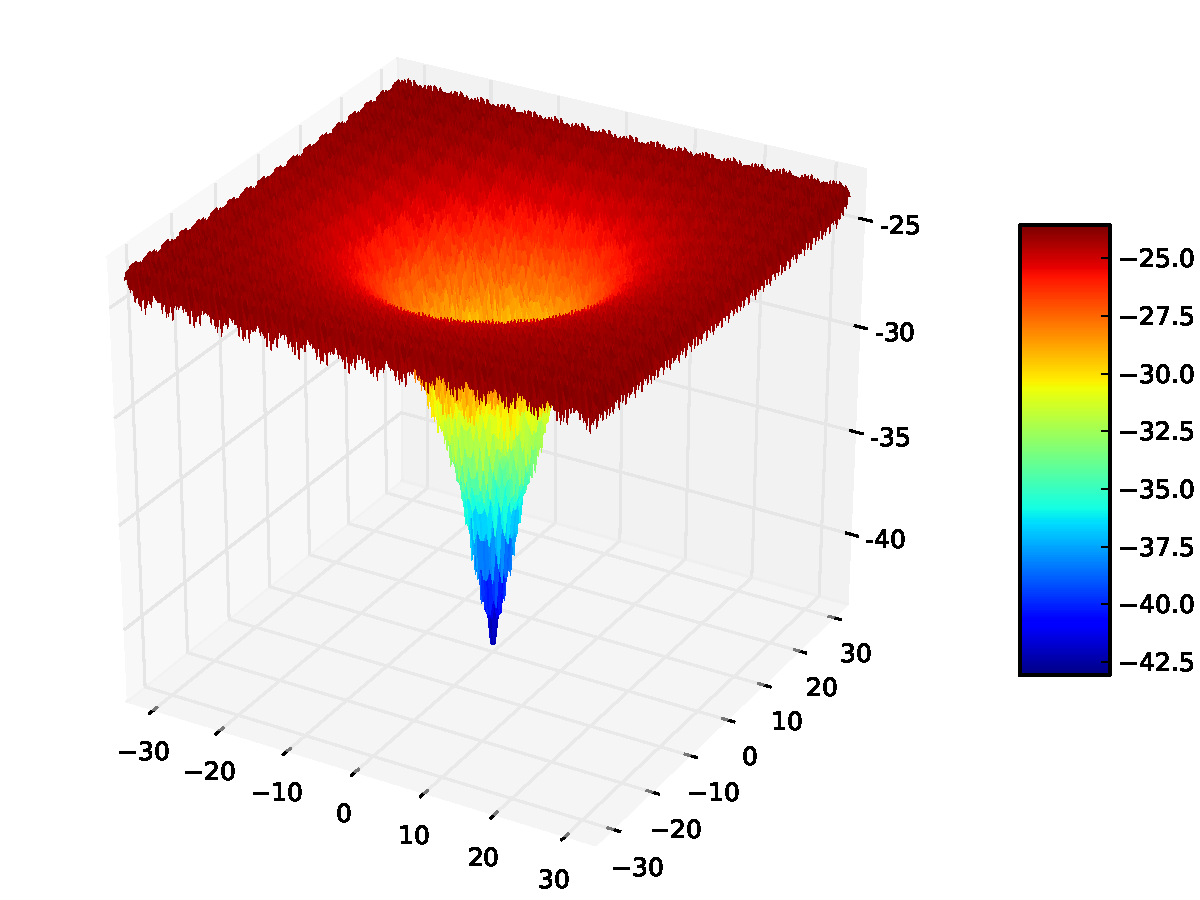
\includegraphics[width=3.0in,height=2.5in]{./Graphs/Ackley.pdf}}
	\caption{Ackley Function}
	\label{fig:AckleyGraph}
\end{figure}
~
\subsubsection{Six-Hump Camel Back Function}
~
\begin{figure}[ht]
	\centering
	\setlength \fboxsep{0pt}
	\setlength \fboxrule{0.5pt}
	\fbox{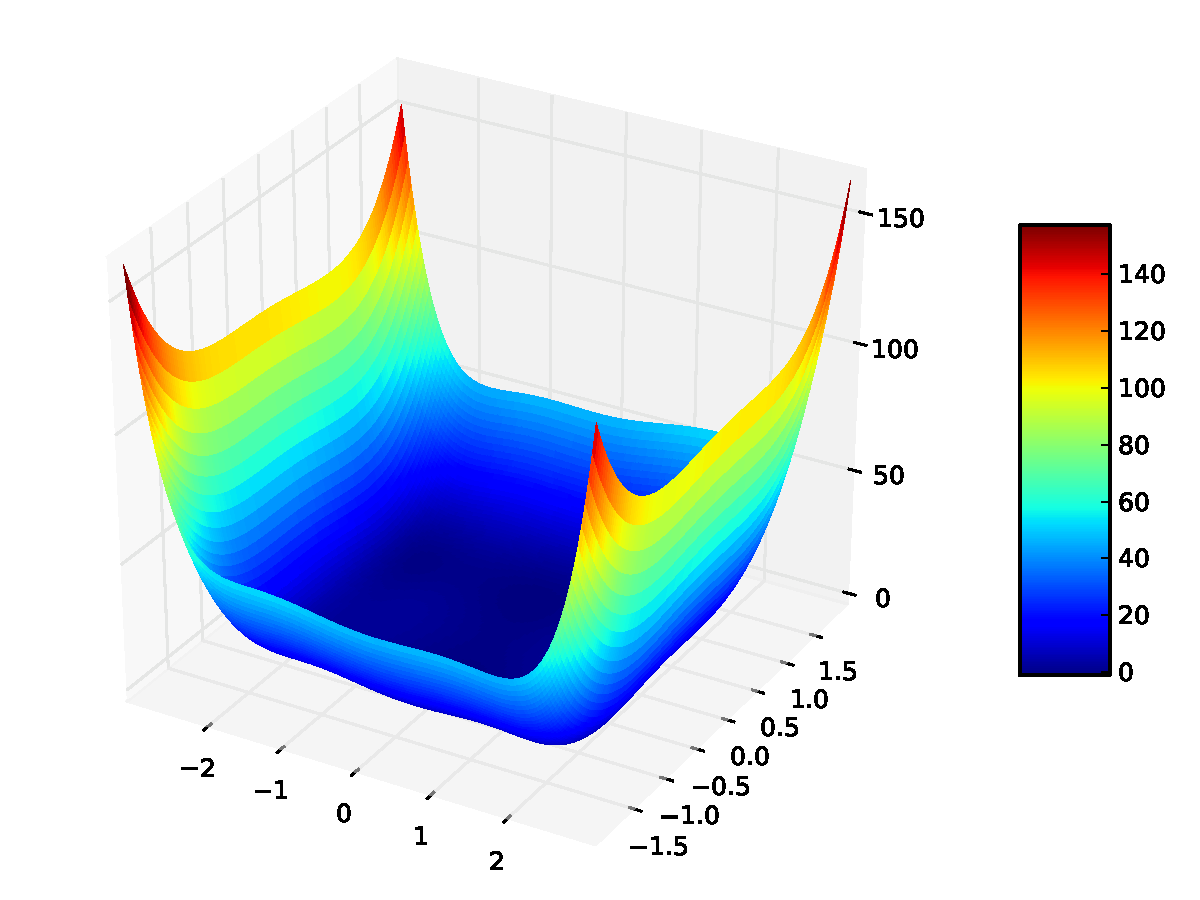
\includegraphics[width=3.0in,height=2.5in]{./Graphs/Camel.pdf}}
	\caption{Six-Hump Camel Back Function}
	\label{fig:CamelGraph}
\end{figure}
~
\subsubsection{Shubert Function}
~
\begin{figure}[ht]
	\centering
	\setlength \fboxsep{0pt}
	\setlength \fboxrule{0.5pt}
	\fbox{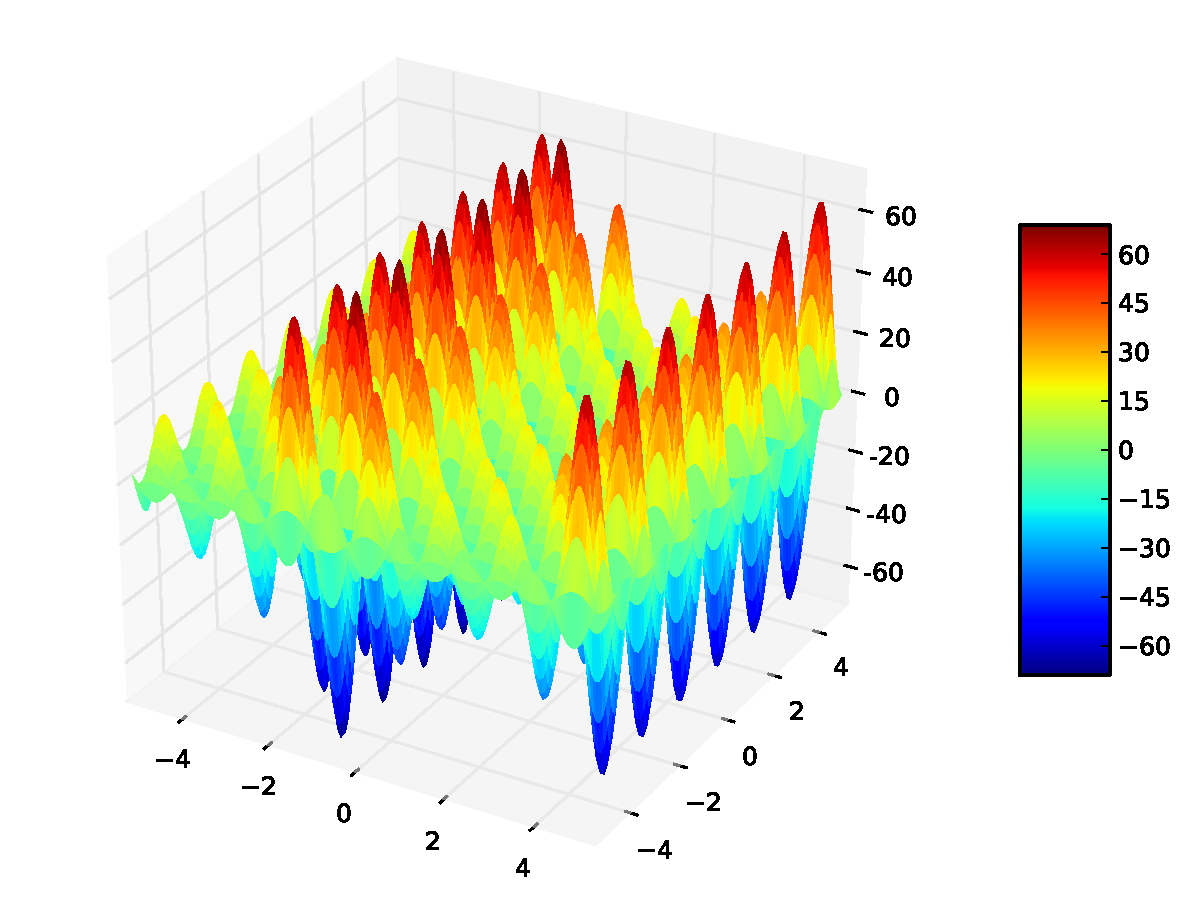
\includegraphics[width=3.0in,height=2.5in]{./Graphs/Shubert.pdf}}
	\caption{Shubert Function}
	\label{fig:ShubertGraph}
\end{figure}
~
\subsubsection{Himmelblau Function}
~
\begin{figure}[ht]
	\centering
	\setlength \fboxsep{0pt}
	\setlength \fboxrule{0.5pt}
	\fbox{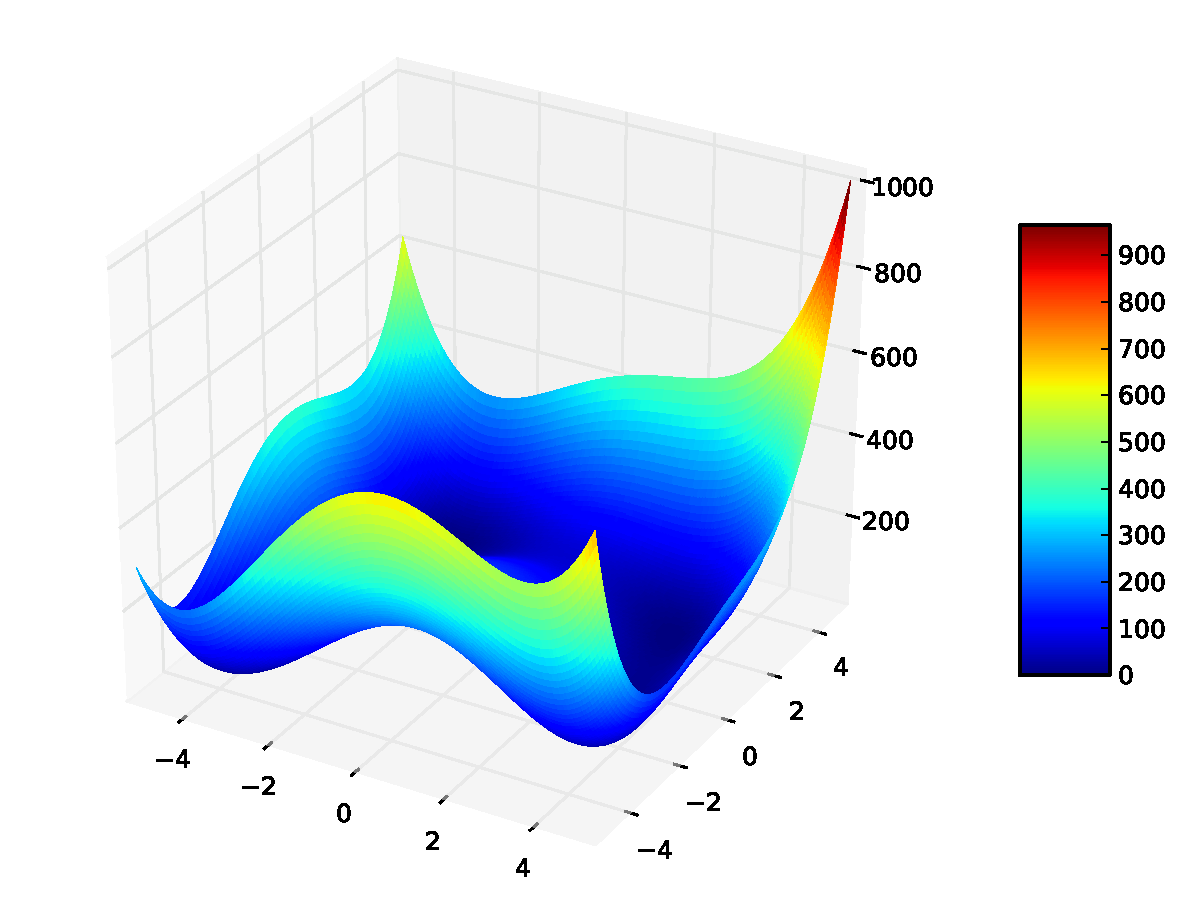
\includegraphics[width=3.0in,height=2.5in]{./Graphs/Himmelblau.pdf}}
	\caption{Himmelblau Function}
	\label{fig:HimmelblaueGraph}
\end{figure}
~
\subsubsection{Rosenbrock Valley Function}
~
\begin{figure}[ht]
	\centering
	\setlength \fboxsep{0pt}
	\setlength \fboxrule{0.5pt}
	\fbox{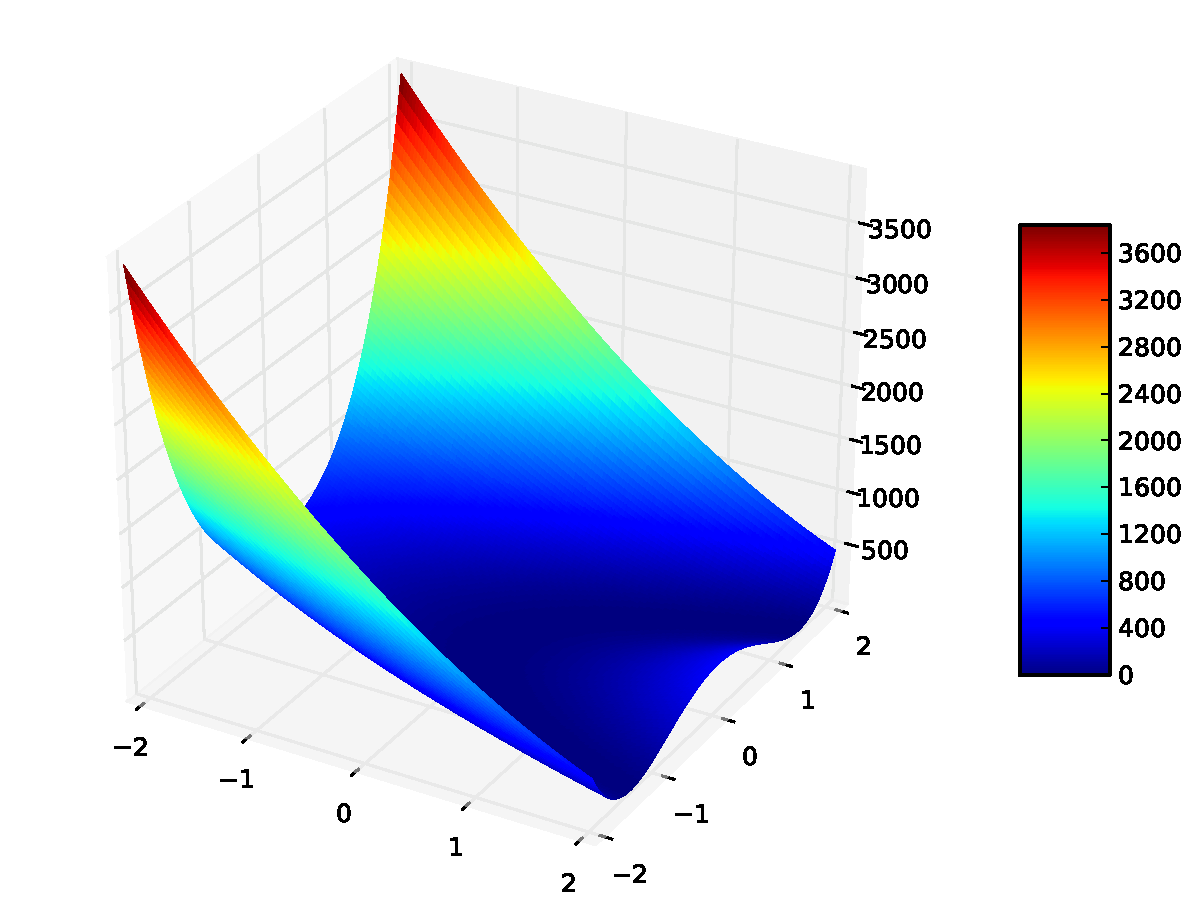
\includegraphics[width=3.0in,height=2.5in]{./Graphs/Rosenbrock.pdf}}
	\caption{Rosenbrock Valley Function}
	\label{fig:Rosenbrock}
\end{figure}
~
\subsubsection{Dropwave Function}
~
\begin{figure}[ht]
	\centering
	\setlength \fboxsep{0pt}
	\setlength \fboxrule{0.5pt}
	\fbox{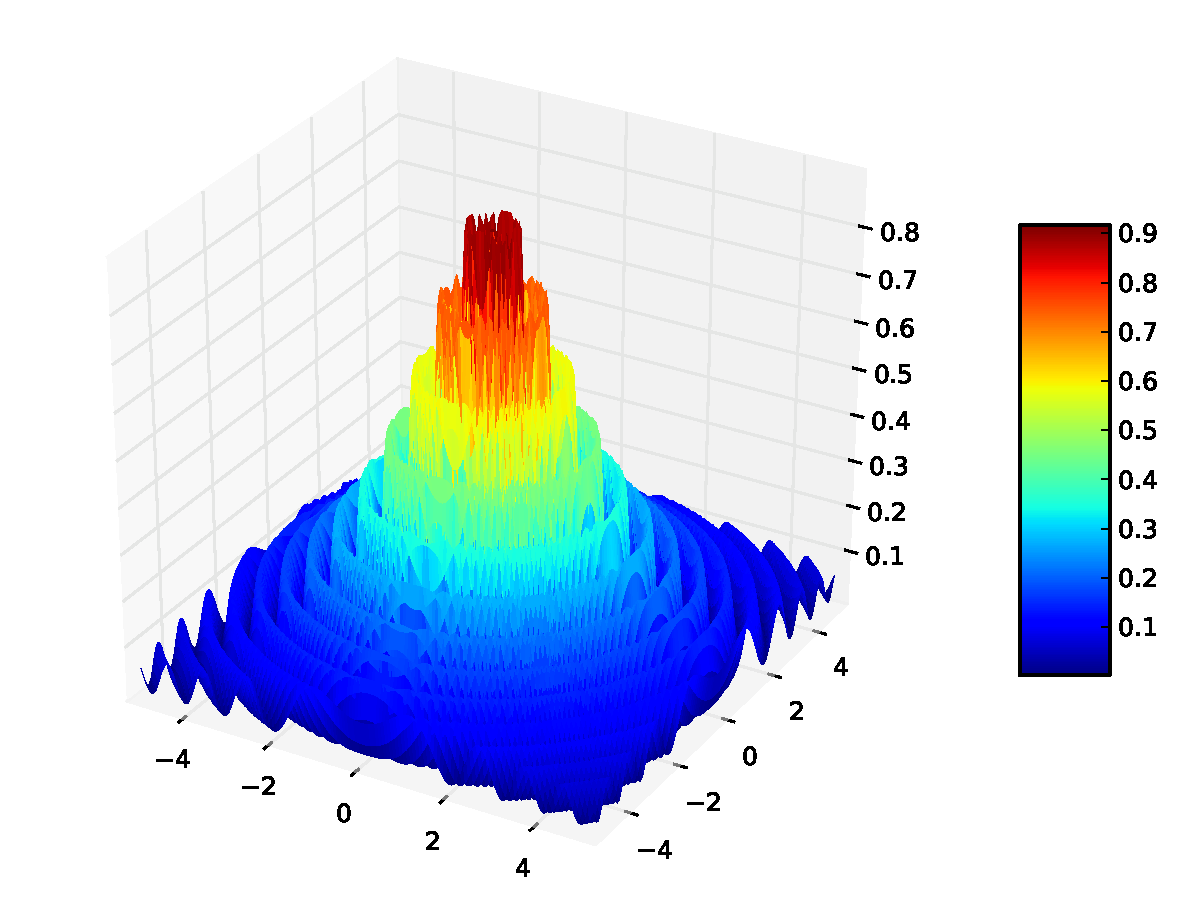
\includegraphics[width=3.0in,height=2.5in]{./Graphs/Dropwave.pdf}}
	\caption{Dropwave Function}
	\label{fig:DropwaveGraph}
\end{figure}
~
\subsubsection{Easom Function}
~
\begin{figure}[ht]
	\centering
	\setlength \fboxsep{0pt}
	\setlength \fboxrule{0.5pt}
	\fbox{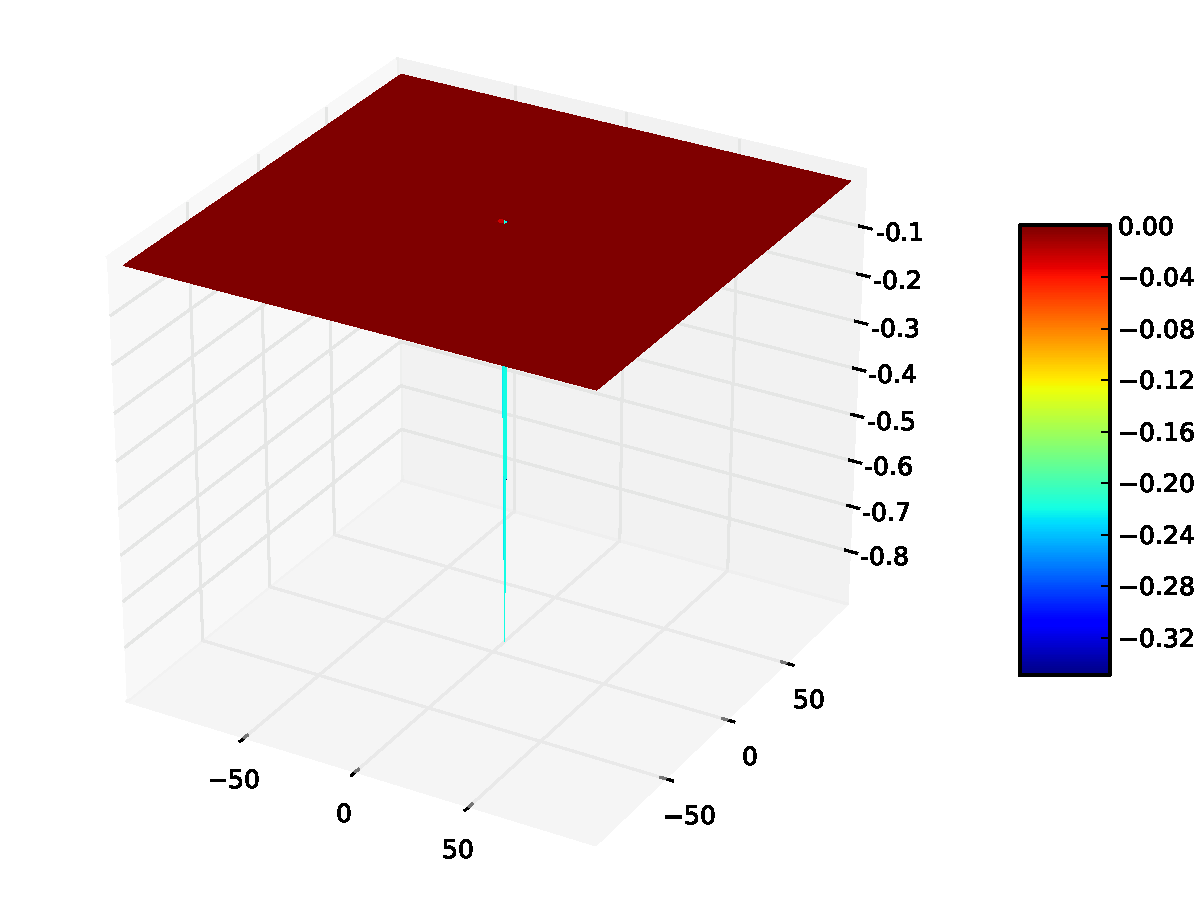
\includegraphics[width=3.0in,height=2.5in]{./Graphs/Easom_-100_+100.pdf}}
	\caption{Easom Function}
	\label{fig:EasomGraph}
\end{figure}
~
\subsubsection{Branin Function}
~
\begin{figure}[ht]
	\centering
	\setlength \fboxsep{0pt}
	\setlength \fboxrule{0.5pt}
	\fbox{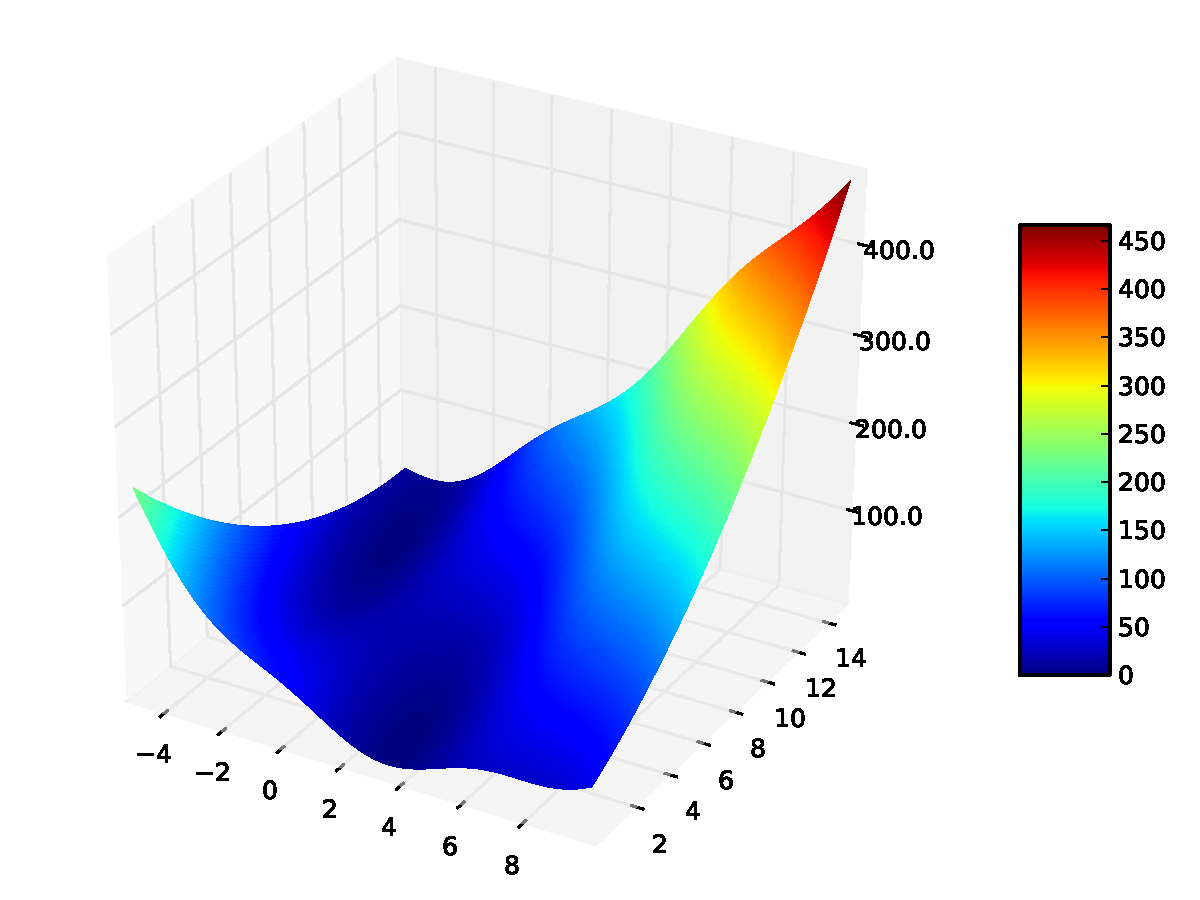
\includegraphics[width=3.0in,height=2.5in]{./Graphs/Branin.pdf}}
	\caption{Branin Function}
	\label{fig:BraninGraph}
\end{figure}
~
\subsubsection{Michalewicz Function}
~
\begin{figure}[ht]
	\centering
	\setlength \fboxsep{0pt}
	\setlength \fboxrule{0.5pt}
	\fbox{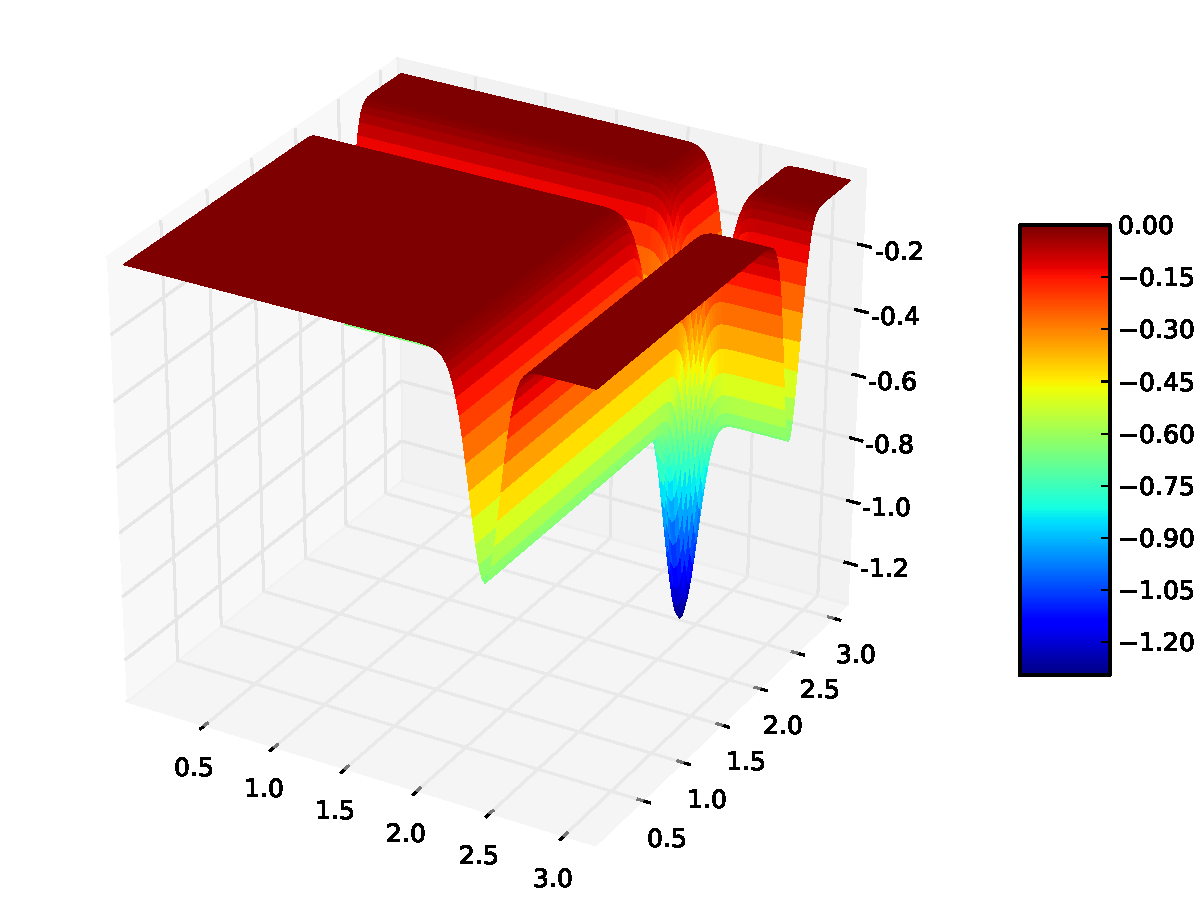
\includegraphics[width=3.0in,height=2.5in]{./Graphs/Michalewicz.pdf}}
	\caption{Michalewicz Function}
	\label{fig:MichalewiczGraph}
\end{figure}
~
\subsubsection{Goldstein Function}
~
~
\begin{figure}[ht]
	\centering
	\setlength \fboxsep{0pt}
	\setlength \fboxrule{0.5pt}
	\fbox{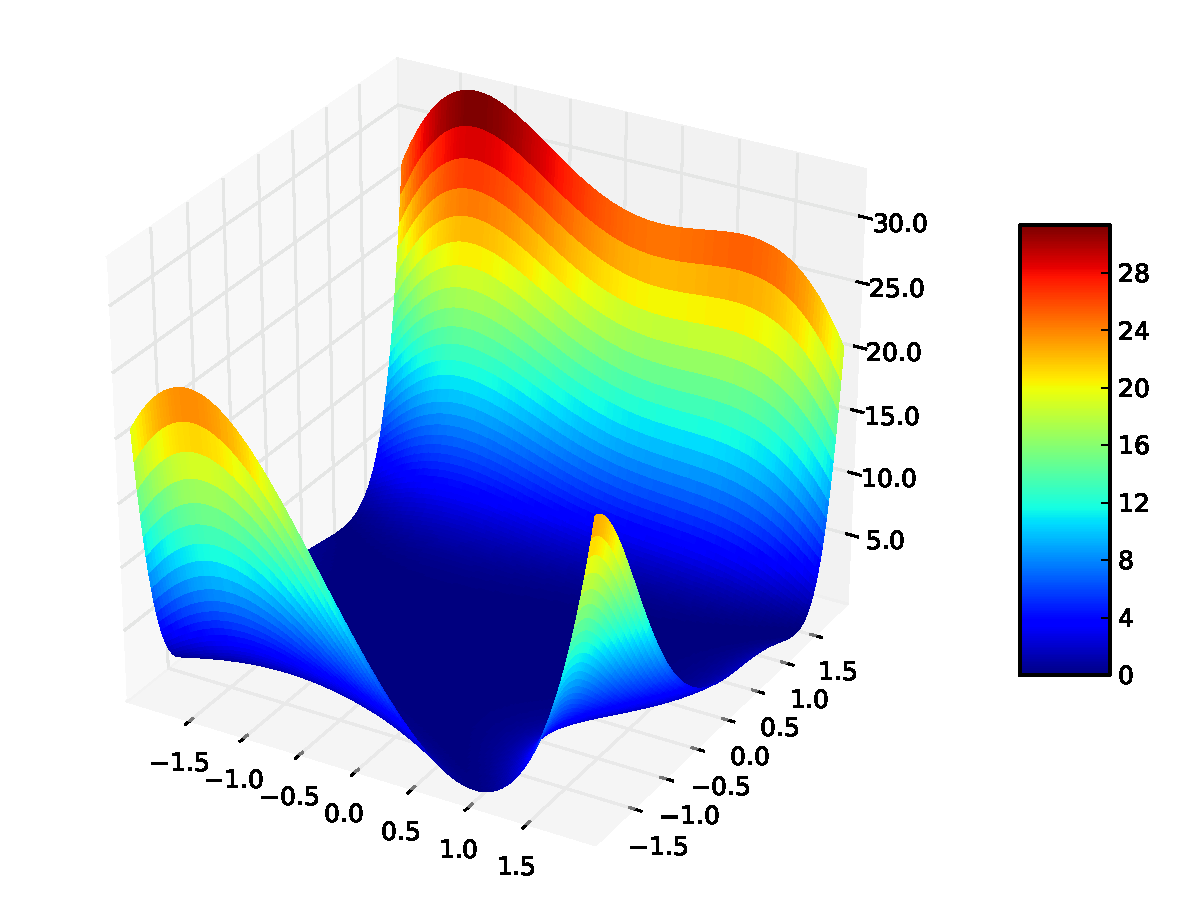
\includegraphics[width=3.0in,height=2.5in]{./Graphs/Goldstein.pdf}}
	\caption{THe Goldstein Function}
	\label{fig:GoldsteinGraph}
\end{figure}
~

\section{Results}
\subsubsection{DeJong's First Function}
\begin{center}
	\begin{tabular}{| c | c |}
	\hline
	Normal PSO & PSO with Inertia \\  \hline
	VALUES & VALUES \\ \hline
	\hline
	\end{tabular}
\end{center}
\subsubsection{Shekel's Foxhole Function}
\begin{center}
	\begin{tabular}{| c | c |}
	\hline
	Normal PSO & PSO with Inertia \\  \hline
	VALUES & VALUES \\ \hline
	\end{tabular}
\end{center}
\subsubsection{Rastrigin Function}
\begin{center}
	\begin{tabular}{| c | c |}
	\hline
	Normal PSO & PSO with Inertia \\  \hline
	VALUES & VALUES \\ \hline
	\end{tabular}
\end{center}
\subsubsection{Schwefel Function}
\begin{center}
	\begin{tabular}{| c | c |}
	\hline
	Normal PSO & PSO with Inertia \\  \hline
	VALUES & VALUES \\ \hline
	\end{tabular}
\end{center}
\subsubsection{Griewank Function}
\begin{center}
	\begin{tabular}{| c | c |}
	\hline
	Normal PSO & PSO with Inertia \\  \hline
	VALUES & VALUES \\ \hline
	\end{tabular}
\end{center}
\subsubsection{Salomon Function}
\begin{center}
	\begin{tabular}{| c | c |}
	\hline
	Normal PSO & PSO with Inertia \\  \hline
	VALUES & VALUES \\ \hline
	\end{tabular}
\end{center}
\subsubsection{Ackley}
\begin{center}
	\begin{tabular}{| c | c |}
	\hline
	Normal PSO & PSO with Inertia \\  \hline
	VALUES & VALUES \\ \hline
	\end{tabular}
\end{center}
\subsubsection{Six-Hump Camel Back Function}
\begin{center}
	\begin{tabular}{| c | c |}
	\hline
	Normal PSO & PSO with Inertia \\  \hline
	VALUES & VALUES \\ \hline
	\end{tabular}
\end{center}
\subsubsection{Shubert Function}
\begin{center}
	\begin{tabular}{| c | c |}
	\hline
	Normal PSO & PSO with Inertia \\  \hline
	VALUES & VALUES \\ \hline
	\end{tabular}
\end{center}
\subsubsection{Himmelblau Function}
\begin{center}
	\begin{tabular}{| c | c |}
	\hline
	Normal PSO & PSO with Inertia \\  \hline
	VALUES & VALUES \\ \hline
	\end{tabular}
\end{center}
\subsubsection{Rosenbrock Valley Function}
\begin{center}
	\begin{tabular}{| c | c |}
	\hline
	Normal PSO & PSO with Inertia \\  \hline
	VALUES & VALUES \\ \hline
	\end{tabular}
\end{center}
\subsubsection{Dropwave Function}
\begin{center}
	\begin{tabular}{| c | c |}
	\hline
	Normal PSO & PSO with Inertia \\  \hline
	VALUES & VALUES \\ \hline
	\end{tabular}
\end{center}
\subsubsection{Easom Function}
\begin{center}
	\begin{tabular}{| c | c |}
	\hline
	Normal PSO & PSO with Inertia \\  \hline
	VALUES & VALUES \\ \hline
	\end{tabular}
\end{center}
\subsubsection{Branin Function}
\begin{center}
	\begin{tabular}{| c | c |}
	\hline
	Normal PSO & PSO with Inertia \\  \hline
	VALUES & VALUES \\ \hline
	\end{tabular}
\end{center}
\subsubsection{Michalewicz Function}
\begin{center}
	\begin{tabular}{| c | c |}
	\hline
	Normal PSO & PSO with Inertia \\  \hline
	VALUES & VALUES \\ \hline
	\end{tabular}
\end{center}
\subsubsection{Goldstein Function}
\begin{center}
	\begin{tabular}{| c | c |}
	\hline
	Normal PSO & PSO with Inertia \\  \hline
	VALUES & VALUES \\ \hline 
	\end{tabular}
\end{center}
